\section{Methodology}

\subsection{Simulated process and study design}

A latent state $\bm{z}_t\in\mathbb{R}^8$ follows a stable mean-adjusted VAR(1), and the four observed variables $\bm{x}_t\in\mathbb{R}^4$ are a nonlinear function of it:
\begin{equation}
\begin{gathered}
\bm{z}_t=\bm{\mu}_t+\bm{\Phi}(\bm{z}_{t-1}-\bm{\mu}_{t-1})+\bm{\eta}_t,\quad
\bm{\eta}_t\sim N(\bm{0},0.2\bm{I}_8),\\
\bm{x}_t=\bm{W}_2\tanh(\bm{z}_t)+\bm{\varepsilon}_t\quad\text{and}\quad
\bm{\varepsilon}_t\sim N(\bm{0},0.05\bm{I}_4),
\end{gathered}
\label{eq:process}
\end{equation}
where $\bm{\eta}_t$ and $\bm{\varepsilon}_t$ are independent Gaussian latent innovations and measurement noise, $\bm{I}_k$ is the $k\times k$ identity, $\bm{\mu}_t=\bm{0}$ in the IC state, $\bm{\Phi}$ is symmetric tridiagonal (diagonal 0.55, adjacent off-diagonals 0.15), $\tanh$ acts componentwise and $\bm{W}_2$ is a fixed $4\times8$ mixing matrix (Appendix~\ref{app:model}). The pre-specified entries of $\bm{\Phi}$ give each latent component persistence and neighbouring components dependence while keeping the process stationary (spectral radius $\approx0.832<1$); as $0.832^{32}\approx0.003$, a 32-observation window spans almost all of this persistence. Each trajectory starts at $\bm{z}_0=\bm{0}$ and discards 500 burn-in steps.
Because the map is nonlinear and $p=4<8$, no linear projection of $\bm{x}_t$ recovers $\bm{z}_t$; the latent
state is never supplied to any model. The fault is a sustained latent mean shift
$\bm{\mu}_t=\delta\bm{v}$ in the fixed direction $\bm{v}=(1,1,0,\dots,0)\T/\sqrt2$, starting at the first
retained observation ($\tau=1$); $\delta$ is the Euclidean size of the shift. Fifteen magnitudes,
$\delta=0.2,0.4,\dots$ and $3.0$, are studied; no other fault type is used.

Five datasets generated from independent random streams have separate roles
(Figure~\ref{fig:pipeline}): In Phase~I, D1 trains the CAE, D2 fits the OC-SVM and D3 estimates the chart moments and calibrates the limits; everything is then frozen and applied unchanged to D4 (independent IC validation) and D5 (OOC evaluation) in Phase~II.

\begin{figure}[!ht]
\centering
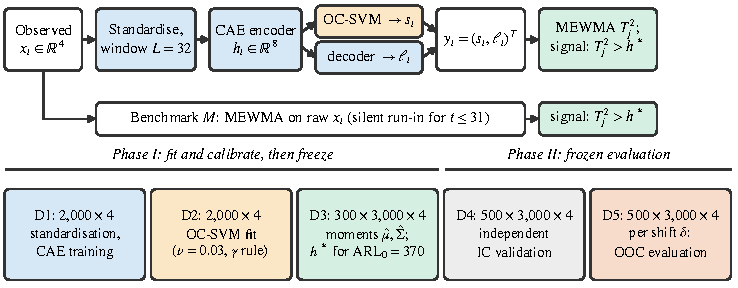
\includegraphics[width=\linewidth]{methodology_pipeline_diagram.pdf}
\caption[Monitoring pipeline and data roles]{Monitoring paths of the hybrid chart $H$ (ablations: $S$
uses $s_t$ only, $R$ uses $\ell_t$ only) and the benchmark $M$ (top), and the roles of the five datasets
(bottom). Box shading marks the dataset on which a stage is fitted or
calibrated.}
\label{fig:pipeline}
\end{figure}

\subsection{Learned components}

\textbf{Windows:} D1 is split chronologically into training rows $[0,1600)$ and validation rows
$[1600,2000)$ before any window is formed. Each variable is standardised with the training-segment
mean and standard deviation, which are then frozen. Windows $\bm{X}_t\in\mathbb{R}^{4\times32}$ of the
$L=32$ most recent standardised observations are formed with stride 1 inside a segment or
trajectory, so a 3000-observation trajectory yields $J=2969$ windows, the first ending at $t=32$.

\textbf{CAE:} The encoder applies two one-dimensional convolutions ($4\to8\to16$ channels), which halve the window length twice, and a linear
bottleneck producing $\bm{h}_t\in\mathbb{R}^q$ with $q=8$; the decoder mirrors it to give the reconstruction $\hat{\bm{X}}_t$ (3180 parameters; layers and optimiser settings in Appendix~\ref{app:model}). The network was trained on
the 1569 D1 training windows to minimise the mean squared reconstruction error, and the checkpoint with
the lowest validation loss (epoch 33) was frozen. The reconstruction error is the summed squared prediction error of the standardised window,
\begin{equation}
\SPE_t=\sum_{c=1}^{4}\sum_{k=1}^{32}\big(X_{t,ck}-\hat X_{t,ck}\big)^2,
\label{eq:spe}
\end{equation}
where $c$ indexes channels and $k$ window positions. The charts use
$\ell_t=\log\max(\SPE_t,10^{-12})$: the floor prevents $\log 0$, and the logarithm puts the error on a scale comparable to the OC-SVM score and removes most of its right skew, without making it Gaussian.

\textbf{OC-SVM:} The 1969 D2 windows are passed through the frozen standardisation and encoder, and
an RBF OC-SVM is fitted to the resulting features $\bm{h}_i$ directly, without further scaling:
\begin{equation}
k(\bm{h},\bm{h}')=\exp\!\big(-\gamma\lVert\bm{h}-\bm{h}'\rVert^2\big),\qquad \nu=0.03\quad\text{and}\quad \gamma=\Big[\operatorname*{median}_{i<j}\lVert\bm{h}_i-\bm{h}_j\rVert^2\Big]^{-1}\approx0.0305,
\label{eq:ocsvm}
\end{equation}
with the median taken over all $\binom{1969}{2}$ pairs. The parameter $\nu$ bounds the fraction of
training windows outside the fitted boundary from above and the fraction of support vectors from
below \citep{scholkopf_estimating_2001}. The score is the negated decision function, $s_t=\rho-\sum_{m=1}^{78}\alpha_m k(\bm{h}_{(m)},\bm{h}_t)$, where $\bm{h}_{(1)},\dots,\bm{h}_{(78)}$ are the support vectors, $\alpha_m$ their dual coefficients and $\rho$ the fitted offset, so a larger $s_t$ means a
more abnormal window.

\subsection{Monitoring charts and calibration}

The hybrid monitoring vector is $\bm{y}_t=(s_t,\ell_t)\T$. For a chart input $\bm{u}_j$ with IC mean $\hat{\bm{\mu}}$ and covariance $\hat{\bm{\Sigma}}$, the MEWMA state
and the plotting statistic are, respectively, \citep{lowry_multivariate_1992}:
\begin{align}
\bm{Z}_j&=\lambda\bm{u}_j+(1-\lambda)\bm{Z}_{j-1},\qquad \bm{Z}_0=\hat{\bm{\mu}},\label{eq:mewma}\\
T_j^2&=(\bm{Z}_j-\hat{\bm{\mu}})\T(c_j\hat{\bm{\Sigma}})^{-1}(\bm{Z}_j-\hat{\bm{\mu}}),\label{eq:t2}
\end{align}
where $j$ indexes monitoring opportunities ($j=1$ at $t=32$), $\bm{u}_j$ is the chart's input at opportunity $j$ (for $H$, $\bm{u}_j=\bm{y}_{j+31}$), $\lambda$ is the smoothing constant and $c_j=\tfrac{\lambda}{2-\lambda}\big[1-(1-\lambda)^{2j}\big]$ is the exact finite-start factor, which is always used. Six configurations of four charts are evaluated (Table~\ref{tab:ic}). The
hybrid chart (denoted as $H(\lambda)$), an OC-SVM--CAE MEWMA chart, monitors $\bm{y}_t$ at the primary $\lambda=0.05$, with $\lambda=0.10$ and $0.20$ as a
sensitivity analysis; the ablations $S(\lambda)$ and $R(\lambda)$ monitor $s_t$ and $\ell_t$ alone, and the benchmark
$M(0.05)$ is a conventional MEWMA on the raw $\bm{x}_t$, each with $\lambda=0.05$. $\hat{\bm{\mu}}$ and $\hat{\bm{\Sigma}}$ are pooled over all $300\times2969$ D3 monitoring vectors ($S$ and $R$ use the matching
entries) and, for $M$, over the aligned raw D3 observations at $t=32,\dots,3000$. Because the hybrid
charts cannot decide before the first window is complete, $M$'s state is updated silently with $\bm{x}_1,\dots,\bm{x}_{31}$ and it first reports at $t=32$ with factor $c_{32}$, so all six charts share the
same 2969 opportunities.

Consecutive windows share 31 of their 32 observations, so the monitored sequences are strongly
autocorrelated (Section~\ref{sec:components}) and $c_j\hat{\bm{\Sigma}}$ is only a reference scaling, not the covariance of $\bm{Z}_j$; without independence, limits derived for independent data lose their nominal \ARL{} properties \citep{lowry_multivariate_1992}. Each limit is therefore calibrated
empirically on D3. For a candidate limit $h$, the run-length (RL) of a trajectory is the first opportunity $j$ with $T_j^2>h$, truncated at $J=2969$, and $\widehat{\ARL}_0(h)$ is the mean RL over the 300 D3 trajectories. As this is a
non-decreasing step function of $h$, the calibrated limit
\begin{equation}
h^*=\min\big\{h\in V:\widehat{\ARL}_0(h)\ge370\big\},
\label{eq:limit}
\end{equation}
where $V$ is the set of values attained by the running maxima of $T_j^2$, is found exactly by bisection, and the chart signals at the first $j$ with $T_j^2>h^*$, where $h^*>0$ is its \UCL{}. The target of 370 is the $\ARL_0$ of a conventional three-sigma Shewhart chart
\citep{ahmed_statistical_2017}.

\subsection{Evaluation design}

If a chart gives no signal by $j=2969$, the RL is recorded as 2969 and flagged as censored by a separate indicator, so each mean is a restricted \ARL{}. D4 yields each chart's independent IC run-lengths, and D5 its OOC run-lengths at the 15 shifts. Because \mbox{$\tau=1$}, the first window is already post-change and a signal at
opportunity $j$ corresponds to $j+31$ post-change observations: $\ARL_1$ is a detection delay
measured from the first permitted decision, the setting in which \citet{lowry_multivariate_1992}
also compared multivariate charts. $H(0.05)$ and $M(0.05)$ monitor the same D5 trajectories, so the
primary comparison is paired,
\begin{equation}
\bar d(\delta)=\frac{1}{500}\sum_{i=1}^{500}\big[\RL_{H,i}(\delta)-\RL_{M,i}(\delta)\big],
\label{eq:paired}
\end{equation}
with standard error $s_d/\sqrt{500}$, where $\RL_{H,i}(\delta)$ is the RL of $H(0.05)$ on D5 trajectory $i$ at shift $\delta$ (similarly for $M$) and $s_d$ the sample standard deviation of the 500 paired differences; a positive $\bar d$ means that the benchmark signalled first.
The design, including every dataset size, was fixed in advance: no model, moment, smoothing constant or limit was changed after D4
or D5 was examined.
